\documentclass{article}
\usepackage{amsmath}
\usepackage{amssymb}
\DeclareMathOperator*{\argmax}{argmax}   
\usepackage{fontspec, xunicode, xltxtra, graphicx,xeCJK,float,pythonhighlight}  
%\setsansfont{楷体} % font name is case-sensitive 
%\setmainfont{楷体} 
\title{一个PyBSP的三十分钟教程}
\author{吴峻峰,张勇瑞\\项目email:solker2015@gmail.com}
\begin{document}
\maketitle
PyBSP是Python语言的扩展,能更好地支持BSP(Bulk Synchronous Parallel)并行计算。本教程假设读者已经熟悉Python编程,同时对并行计算有一些了解(最起码知道MPI吧)。

\section{BSP简介}
BSP计算模型是设计并行程序的一种极先进的方法,不但能有效避免传统并行编程工具MPI和PVM中常见又可恶的消息传递死锁现象,而且能在降低编程难度的同时保持非常高的并行计算效率。BSP能做到这些,关键在于,BSP程序设计思想是批量同步 (Bulk synchronous),所有通信都由这种同步自动完成,不但完全避免程序员编程不小心造成的死锁,而且类似于物流企业用批量运输来降低运营成本、提高物流效率,批量同步降低了通信成本,提高了通信效率。

BSP的批量同步能实现,主要在于超步(superstep)概念的引入。一 个BSP程序同时具有水平和垂直两个方面的结构。从垂直上看,一个BSP程序由一系列串行的超步组成,如图所示:
\begin{figure}[H]
\centering
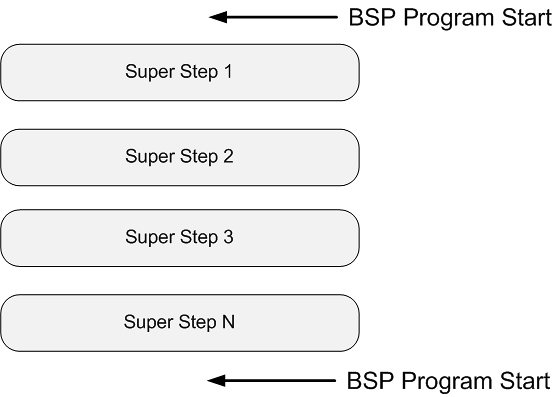
\includegraphics[width=0.6 \textwidth]{hama-bsp.jpg}
\caption{BSP模型纵向分解}
\end{figure}
这种结构类似于一个串行程序结构。从水平上看, 在一个超步中, 分三个阶段:第一阶段是所有的进程并发执行局部计算(local computation);第二阶段是各自激发全局通信(Communication),以解决下个超步计算对异地数据的依赖关系;第三阶段是全局栅栏同步(Barrier Synchronous),以确保所有通信完成后再进入下个超步。这种水平分解如下图所示:
\begin{figure}[H]
\centering
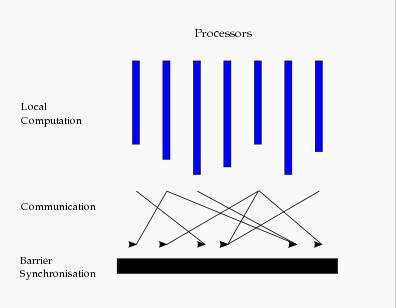
\includegraphics[width=0.6 \textwidth]{hama-bsp2.jpg}
\caption{BSP模型横向分解}
\end{figure}

\section{PyBSP的基本BSP操作}
下面这个例子是用来介绍基本BSP操作的。这个例子首先创建了一些Python对象和numpy数组,然后把它们打包发给其他进程,使得在同步之后,其他进程可以从接收到的包裹中解包出这些对象和数组,并打印出它们的内容。
\begin{python}
import bsp #这是我们的BSP模块
import numpy
import math

procCount=bsp.procCount() # 取出参与并行计算的进程数
myProcID=bsp.myProcID() # 取出当前进程的编号
partnerID = 1^myProcID # 为简单起见,每个进程都先确定通信伙伴

s1 = [1,(2,3,4),[5,(5,6)],{7:[1,2],8:9}] # 随便做个python对象做测试
s2 = (3,5,'123','hello world!') # 另一个随意做出来的对象
bsp.fromObject(s1,'obj.s1') # 把对象s1打包为包裹obj.s1
bsp.fromObject(s2,'obj.s2') # 把对象s2打包为包裹obj.s2

# 下面也是乱做两个numpy数组来做测试
a1 = numpy.ndarray([2,3,3],dtype='f8') 
a2 = numpy.ndarray([10])
for i in range(3):
    for j in range(3):
        a1[0][i][j] = i+j
        a1[1][i][j] = i-j
for k in range(10):
    a2[k] = math.cos(k)
    
# 用bsp.fromNumpy可以打包numpy数组
# (其实也可以用bsp.fromObject,但bsp.fromNumpy是高度优化的)
bsp.fromNumpy(a1,'num.a1')
bsp.fromNumpy(a2,'num.a2')

# 用bsp.toProc来请求发送包裹到指定的进程
# 这里指定了前面的通信伙伴为目的地
# 其实也可以任意指定其它进程
bsp.toProc(partnerID,'obj.s1') 
bsp.toProc(partnerID,'obj.s2')
bsp.toProc(partnerID,'num.a1')
bsp.toProc(partnerID,'num.a2')

# 做个全局同步,完成这个超步的所有通信
bsp.sync('hello') 
# hello是个随意给的校验口令。校验口令是为了防止同步的错误匹配。
# 仅当通信两边程序的校验口令一致时,全局同步才是正确匹配。
# 当bsp发现错误匹配的同步时,会向用户报告错误,并终止所有进程。

# 从包裹中取出从通信伙伴发过来的对象和Numpy数组
t1=bsp.toObject(bsp.fromProc(partnerID)['obj.s1'])
t2=bsp.toObject(bsp.fromProc(partnerID)['obj.s2'])
b1=bsp.toNumpy(bsp.fromProc(partnerID)['num.a1'])
b2=bsp.asNumpy(bsp.fromProc(partnerID)['num.a2'])
# 请留意上一行中的asNumpy。其实,bsp的包裹都是用numpy数组来存储数据的。
# 因此,既可以用bsp.toNumpy来复制一个numpy数组,也可以用bsp.asNumpy来
# 直接访问包裹内容。
# 然而(!!),bsp.asNumpy的缺点(其实很多时候是优点)是,如果对其返回
# 数组进行写入数据的操作,包裹的内容会直接改变!!

# 打印这些发过来的对象和数组
print 't2 = ', t2
print 't1 = ', t1
print 'b1 = ', b1
print 'b2 = ', b2
\end{python}

假设上述Python程序文件是test目录下的ex1.py,而PyBSP的可执行文件是当前目录下的pybsp,则下面这个命令可以用来运行上面这段程序:
\begin{verbatim}
$ mpirun -np 4 .\pybsp test\ex1.py
\end{verbatim}


\section{进阶BSP操作:包裹共享与按需访问}
其实我们不一定要把整个包裹发给目的地进程。很多时候,更好的选择是,把包裹放在共享的地方,让其它进程根据需要取包裹里的任意部分数据。PyBSP提供了一个Globalize-Privatize的机制,globalize是把所有进程的同名包裹共享并组合成为全局数组,privatize是取消共享。请看下面的例子(还是4个进程):
\begin{python}
import bsp
import numpy
import math

# 这个程序需要二维阵列(n1Dim,n1Dim)个进程,其中n1Dim是整数
# 下面,我们把这些进程排成方阵,i0、i1是进程的坐标
nProcs = bsp.procCount()
myProcID = bsp.myProcID()
n1Dim = int(math.floor(math.sqrt(nProcs)))
i0 = myProcID / n1Dim
i1 = myProcID % n1Dim

# 为了创造全局数组,我们先创建局部的包裹
# 下面的bsp.createArray是先创建一个numpy数组,然后把它打包成包裹
bsp.createArray('arr.a1','f8',[10,10])
# 初始一下包裹里面的数据
a1=bsp.asNumpy('arr.a1')
for i in range(10):
    for j in range(10):
        a1[i][j] = i0+i1+i+j

# 好了,现在可以组合全局数组了
# bsp.globalize是用来共享包裹,并把包裹组合成全局数组的。
# 其第一个参数是参与组合的第一个进程的编号,这里我们选了0。
# 第二个参数是参与组合的进程所排的阵列,我们选了n1Dim*n1Dim。
# 从第三个参数开始,是要在这个进程阵列里组合全局数组的包裹名。
# 这里我们只组合了arr.a1,组合后可以用arr.a1@global来访问全局数组。
# 如果有第4个参数,并且是arr.a2,则同时也组合出arr.a2@global。
bsp.globalize(0,(n1Dim,n1Dim),'arr.a1')
# 组合好后,可以根据组合阵列和包裹的大小来计算出全局数组的大小。
# 例如这里,arr.a1@global的大小是(n1Dim*10, n1Dim*10)。
# 注意,不同进程上的包裹大小可以不一样,只要能组合在一起就可以了。
# 例如,如果进程0上包裹大小为(3,3),进程1上为(3,4),进程2上为(4,3),
# 进程3上为(4,4),那么这四个进程用
# bsp.globalize(0,(2,2),'XXX')
# 组合出来的全局数组大小就是 (7,7).

# 创建一个索引集,用来指定访问全局数组哪些范围
inds1=bsp.createRegionSet(([[5,5],[2,0]],[[14,14],[11,9]]));
# 这里用bsp.createRegionSet创建了一个包含两个区域的索引集,
# 一个区域是(5至14,5至14),另一个是(2至11,0至9)。
# 下面继续...
\end{python}
在继续这个例子之前先打个岔,我们现在决定一下究竟是要从arr.ar1@global拿数据呢还是向它里面更新数据。假设我们是要拿数据的,那么,我们就:
\begin{python}
# 创建一个(2,10,10)大小的包裹来准备存放取得的数据
bsp.createArray('arr.a2','f8',[2,10,10])

# 用前面创建的索引集来取得数据,并指定存入arr.a2
bsp.requestTo('arr.a2','arr.a1@global',inds1)
bsp.sync('just for fun!!')

# 打印取出来的数据
if myProcID == 0:
    a2 = bsp.asNumpy('arr.a2')
    print a2
\end{python}
反之,如果是要向arr.ar1@global更新数据的,我们就:
\begin{python}
# 创建一个(2,10,10)大小的包裹来存储要更新的数据
bsp.createArray('arr.a2','f8',[2,10,10])
# 准备好要更新的数据
a2=bsp.asNumpy('arr.a2')
for i in range(2):
    for j in range(10):
        for k in range(10):
            a2[i][j][k] = 1.0

# 用前面创建的索引集来更新数据,指定新数据来自arr.a2
bsp.updateFrom('arr.a2','+','arr.a1@global',inds1)
bsp.sync('just for fun!!')

# 打印更新后的数组
if myProcID == 0:
    print a1
\end{python}

\section{关于PyBSP的内存管理}
由于PyBSP的包裹投递服务是跨进程的,所以如果有包裹不需要了,必需用如下的语句来删除,python的垃圾回收机制不能自动回收包裹:
\begin{python}
bsp.delete('包裹1','包裹2',...,'包裹k')
\end{python}
其中k不超过10。另外要注意,如果有多个包裹有相同的前缀(前缀是用.来隔开的),例如arr.a1和arr.a2有相同的前缀arr,那么
\begin{python}
bsp.delete('arr')
\end{python}
就可以同时删除arr.a1和arr.a2。此外,如果其中有一些包裹是已经globalize的,例如arr.a1,就必须先用
\begin{python}
bsp.privatize('arr.a1')
\end{python}
来私有化这个包裹,再调用bsp.delete。最后,索引集也是包裹投递服务的要素,因此同样道理,要用如下语句来删除:
\begin{python}
bsp.delete(索引集变量)
\end{python}

\section{关于不同类型的索引集}
PyBSP支持四种类型的一至七维索引集:
\subsection{点序列索引集}
\begin{python}
inds1=bsp.createPointSet([[5,5],[2,0]])
\end{python}
这样就用bsp.createPointSet创建了一个包含两个点的二维点序列索引集,这两个点分别是(5,5)和(2,0)。

\subsection{点张量索引集}
\begin{python}
inds1=bsp.createPointSet([5,3],[2,4,7])
\end{python}
这样就用bsp.createPointSet创建了一个包含六个点的二维点序列索引集,这六个点分别是(5,2),(5,4),(5,7),(3,2),(3,4),(3,7),这是由x1的两个值和x2的三个值通过张量组合在一起的。

\subsection{区域序列索引集}
\begin{python}
inds1=bsp.createRegionSet(([[5,5],[2,0]],[[14,14],[11,9]]));
\end{python}
这样就用bsp.createRegionSet创建了一个包含两个区域的二维区域序列索引集,一个区域是(5至14,5至14),另一个是(2至11,0至9)。

\subsection{区域张量索引集}
\begin{python}
inds1=bsp.createRegionSet(([5,3],[7,8]),([2,4,7],[5,6,9]))
\end{python}
这样就用bsp.createRegionSet创建了一个包含六个区域的二维区域张量索引集,这些区域分别是(5至7,2至5)、(5至7,4至6)、(5至7,7至9)、(3至8,2至5)、(3至8,4至6)、(3至8,7至9),它们是通过(lo1,up1)的两个一维区域和(lo2,up2)的三个一维区域张量组合而成。 

\end{document}